\documentclass[../thesis]{subfiles}
\graphicspath{{\subfix{../figures/}}}

\begin{document}
\chapter{Implementation}\label{ch:implementation}

\lettrine[lines=3]{\textcolor{Maroon}{R}}{elying} on the foundations of \SEE{} and the \glsentrylong{lsp} established in the previous chapter, we can now turn to the core part of this thesis:
The integration of \gls{lsp} into \SEE{}, with a special focus on how to build \glspl{city} using \gls{lsp}'s \glspl{capability}.
We will start by briefly going over some preliminary changes to both \SEE{} and the \gls{lsp} specification.
Then, we will spend a good chunk of this chapter specifying and explaining the algorithm which "converts" \gls{lsp} information into \glspl{city}, before looking into how additional \glspl{capability} can be integrated into \SEE{}'s \glspl{city} and \glspl{window} specifically.
Finally, we will conduct a brief technical evaluation, with a more thorough user study following in the next chapter.

\section{Preliminary Changes}
As promised in the preceding paragraph, we will first quickly list some preparations.

\subsection{Specification Cleanup}
While familiarizing myself with the \gls{lsp} specification, I noticed and fixed a few small issues along the way.
Most of these were of a formal nature (\eg, spelling, grammar, formatting, consistent usage of terms), some were fixing incorrect TypeScript syntax in the definition of \gls{lsp}'s data models.
The rest of the changes were related to the so-called snippet grammar.

In the context of \gls{lsp}, snippets are in essence string templates that are inserted on certain completions (see \cref{subsec:unplanned}), with some designed parts being filled in by the programmer on insertion.
There are also parts that can be filled in by certain values (\eg, the file name), which can themselves be transformed using regular expressions.\footnote{
	I am skipping over some additional features and details here because this is not that relevant a \gls{capability} for us---to get the full picture, see \web{https://microsoft.github.io/language-server-protocol/specifications/lsp/3.18/specification/\#snippet\_syntax}{2024-10-10}.
}
The complexity of the combinations of all these features increase the possibility of misunderstandings, which is why the snippet's grammar has been formally specified in \gls{ebnf}.
However, as it was written down in the specification, the grammar had a few problems that I have fixed.
Three notable examples are:
\begin{itemize}
	\item Some alternatives were incorrectly grouped, contradicting the explanatory text above them.
	      Also, the rules on how and when control characters had to be escaped were inconsistent with the surrounding text.\footnote{
		      This has lead to confusion in some projects making use of snippets.
		      See, for example, \web{https://github.com/neovim/neovim/issues/30495}{2024-10-10}.
	      }
	\item The grammar contained some string transformations that were unexplained in the text.
	      Since the \gls{lsp} specification is based on \gls{vscode}, I added explanations to the text based on what these transformations did in \gls{vscode}'s source code.
	\item Finally, there were ambiguities present in the grammar that led to \textsf{FIRST}/\textsf{FOLLOW} conflicts.
	      I have rewritten the grammar to eliminate these, and it should now be $LL(1)$-parseable~\cite[222--224]{aho2007}.

\end{itemize}


I have submitted these fixes as a pull request\footnote{\web{https://github.com/microsoft/language-server-protocol/pull/1886}{2024-10-10}}.
After addressing the resulting code review, it has been merged, and the changes will be incorporated in the upcoming 3.18 release of the specification.

\subsection{Preparing SEE}
There was not much I had to do in terms of getting \SEE{} ready, so this section will be very short:
\begin{itemize}
	\item I have integrated the OmniSharp \gls{lsp} C\# library\footnote{
		      Available at \web{https://github.com/OmniSharp/csharp-language-server-protocol}{2024-10-11}
	      } into \SEE{}, which we will leverage in the subsequent sections so that we can use \gls{lsp} without needing to worry about \gls{jrpc} encoding, data models, and so on.
	\item \Glspl{window} have previously been made editable by \textcite{moritz} in his bachelor thesis, also enabling collaborative editing over the internet.
	      I unfortunately had to remove these changes because they did not work anymore in the current version of \SEE{}, and additionally caused a lot of complexity overhead in the \gls{window} implementation that would have made the \gls{lsp} integration much harder to accomplish.
	\item Finally, the attribute space $\mathcal{A}$ in \SEE{} did not allow for \glspl{range} of the form \gls{lsp} needs, so I had to replace the existing attributes (which track the line and column, but not a full range) with a proper set of \gls{range} attributes.
	      In \cref{subsec:graph}, we have introduced this as a single \tt{Source.Range} attribute, but in reality, there are four \gls{range} attributes---one per member of the decomposed form.
	      We will ignore this reality for the rest of this thesis and act like the \gls{range} is a single attribute, that is, for all project graphs with nodes $V$ and attributes $a$, it holds that $\{a(v, \tt{Source.Range}) \mid v \in V \land (v, \tt{Source.Range}) \in \mathrm{dom}(a) \} \subseteq \mathcal{R}$.
\end{itemize}

All of these changes have been made across two pull requests to \SEE{}.\footnote{
	\url{https://github.com/uni-bremen-agst/SEE/pull/687} and \web{https://github.com/uni-bremen-agst/SEE/pull/715}{2024-10-11}.
}

\section{Generating Code Cities using LSP}\label{sec:generate}
In this section, we will examine the centerpiece of this thesis:
The algorithm with which \glspl{city} can be generated using the \glsentrylong{lsp}.
While going over how the algorithm works, we will take a quick look at \glspl{kdtree} and how they relate to the algorithm, before finally taking a look at what the import process looks like in practice in \SEE{}.

\subsection{Algorithm}

We will take a look at the algorithm in a generalized and programming language independent form here.
In this form, the algorithm takes as input a set of source code documents, as well as a family of \gls{lsp} functions belonging to a specific instantiation of a \gls{ls}.
These functions will be used to analyze the documents and extract the required information from them.
The output of the algorithm, then, is a graph representing the given software project.

\begin{figure}
	\begin{center}
		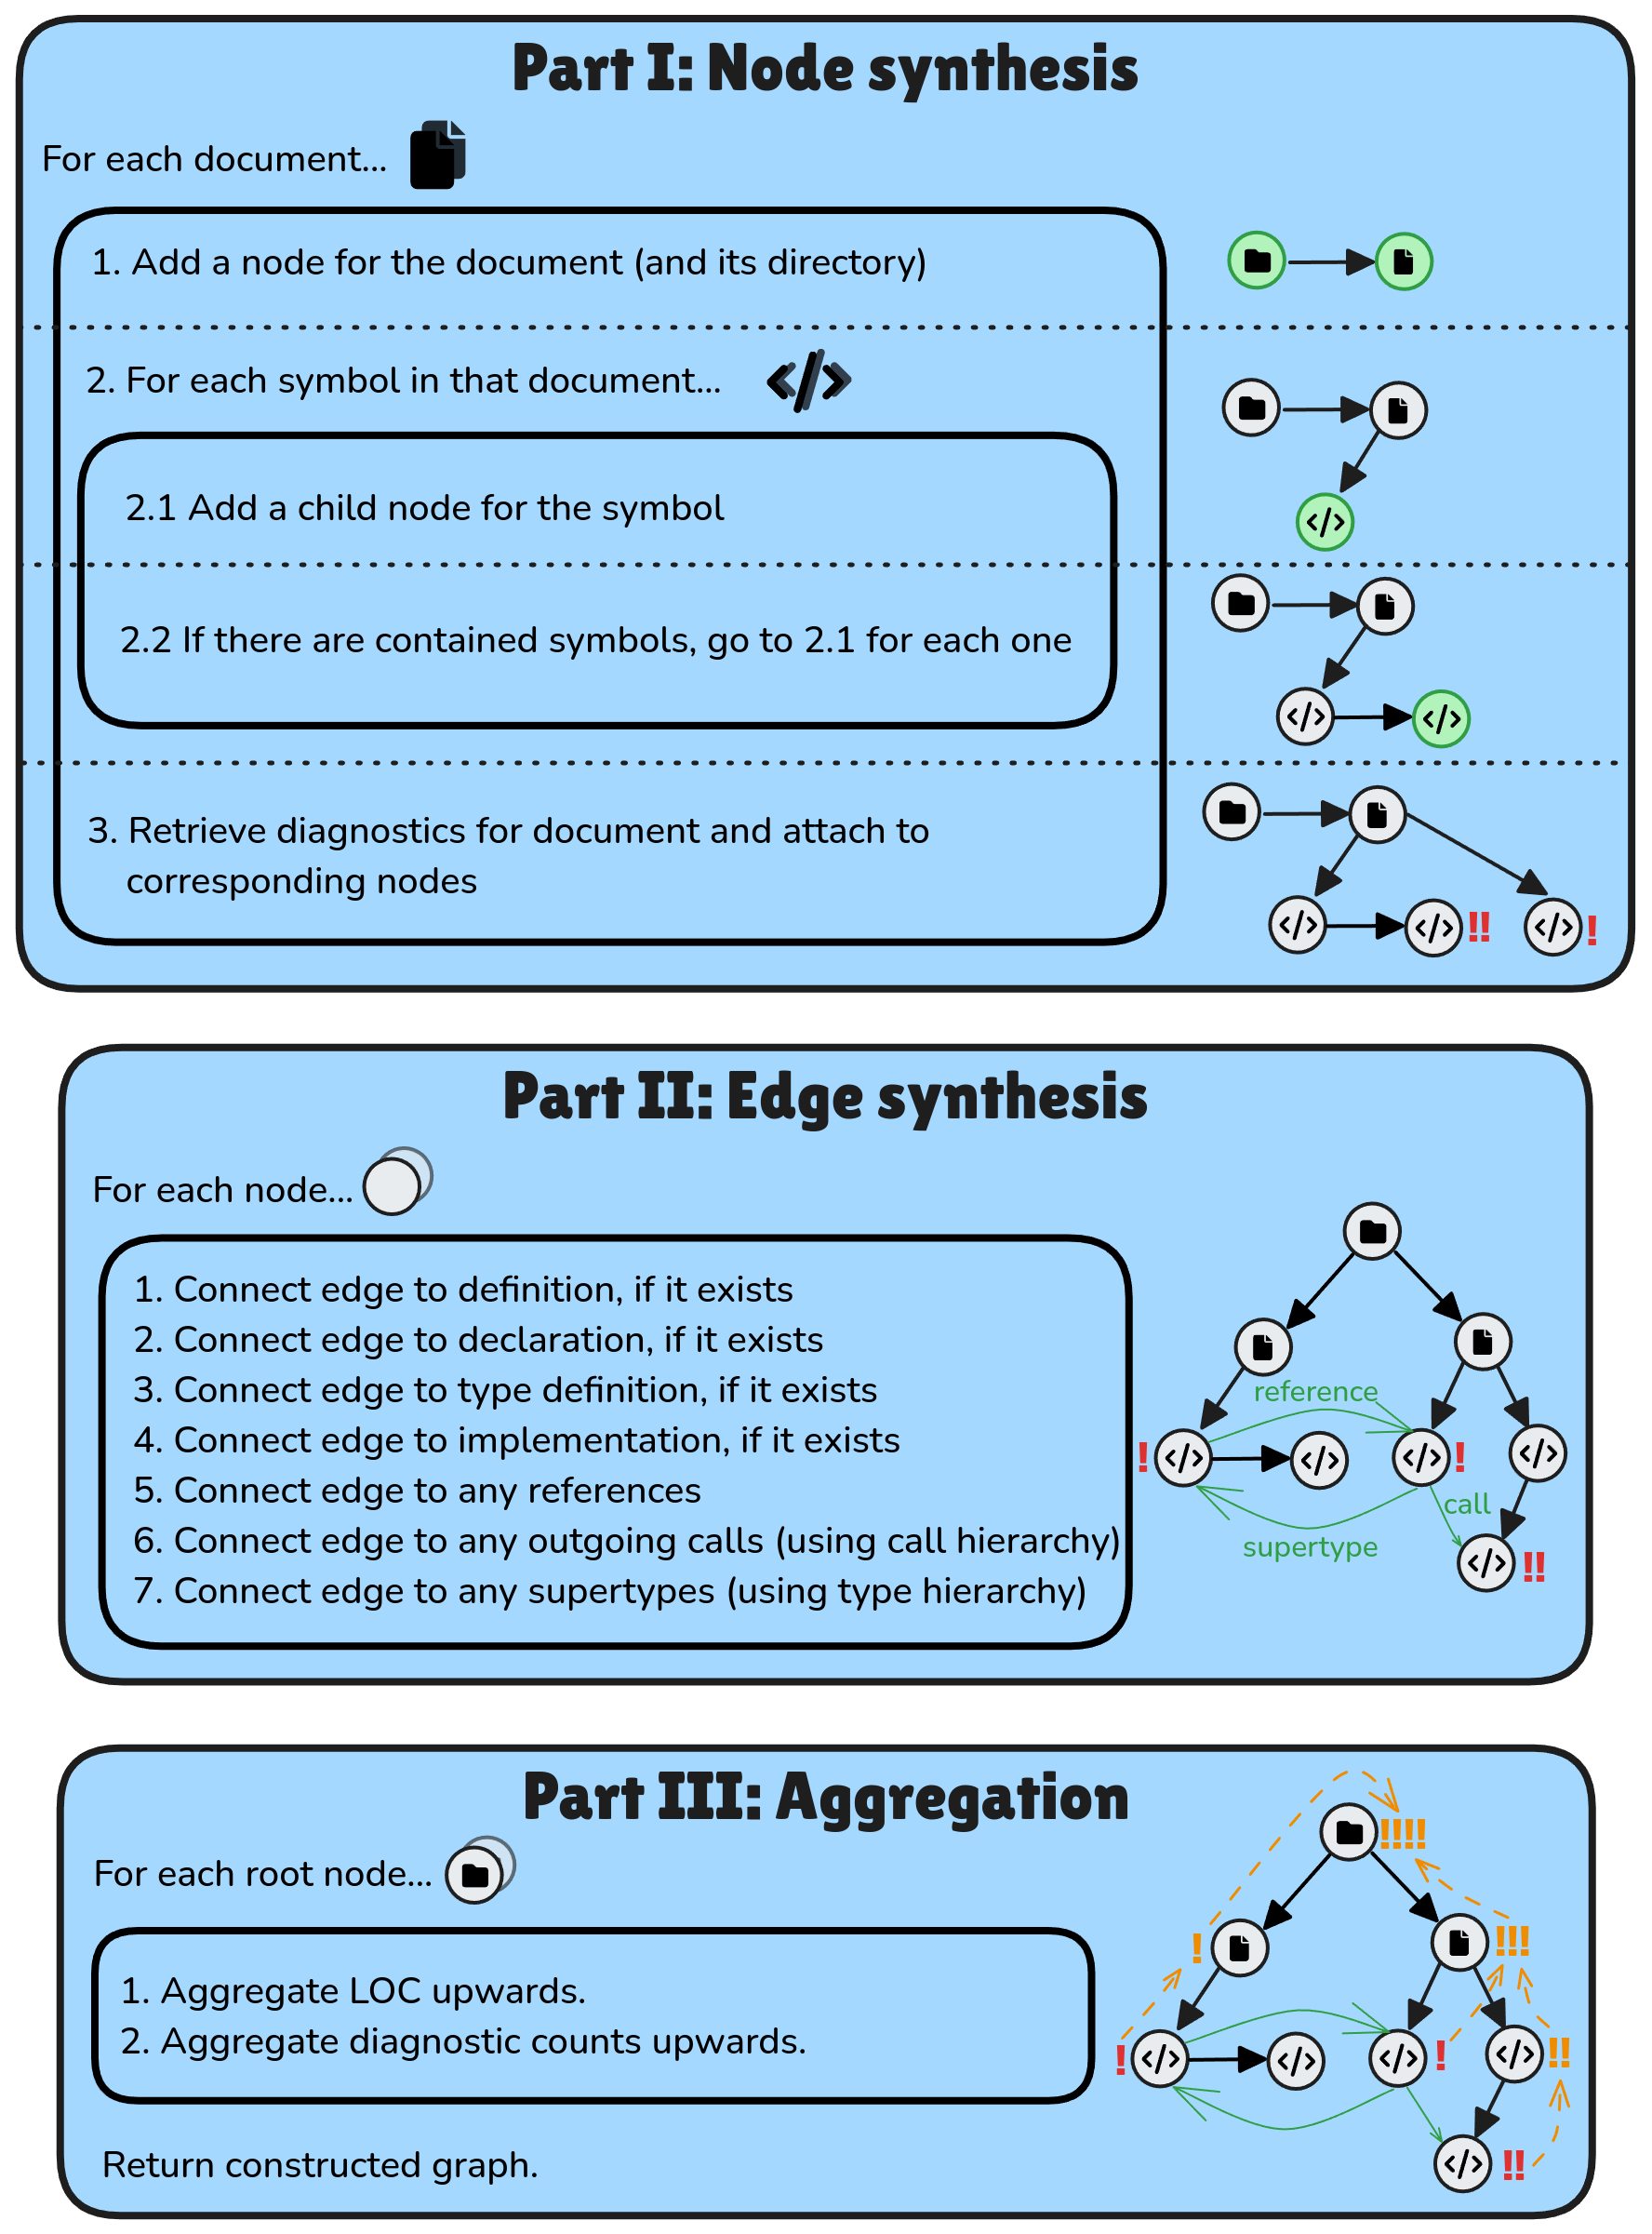
\includegraphics[width=0.95\textwidth]{overview_algorithm}
	\end{center}
	\caption{A high-level overview of the basic steps of the algorithm.}\label{fig:alg_overview}
\end{figure}
\fxnote{Replace diagram sketch with TikZ picture.}

Before diving into the specifics of \emph{how} the algorithm works, it may help to take a look at the diagram in \cref{fig:alg_overview}, which gives us a high-level overview of \emph{what} it does.
To summarize, the steps can be broken down into three major parts:
\begin{enumerate}[label=\bfseries\Roman*]
	\item \textbf{Node synthesis:} Here, we create the graph's nodes and combine them together into a hierarchy.
	      \begin{enumerate}[label=\arabic*.]
		      \item We recreate the parts of the filesystem hierarchy that are relevant to the given documents (\ie, directories the documents are contained in and their relation to each other).
		      \item For each code symbol within that document, a node will be created as a child to the document.
		            Any symbols contained within that symbol are recursively added in the same manner as a child to their parent nodes.
		      \item Finally, we will pull diagnostics for the document\footnote{
			            In the actual algorithm, we cannot rely on pulling diagnostics alone, since only few \glspl{ls} support this.
			            Instead, we will collect pushed diagnostics in the background and handle them all at once at the very end.
		            } and attach their counts to the nodes they correspond to.
	      \end{enumerate}
	\item \textbf{Edge synthesis:} Here, we connect the nodes by creating edges between them.
	      To do this, we go over each node, using \gls{lsp} functions to check for definition locations, references, and so on, and then determine which of our existing nodes best corresponds to that location.
	      This turns out to be the most difficult and complex part of the algorithm to implement efficiently, as we will later see.
	\item \textbf{Aggregation:} Finally, we want to aggregate \gls{loc} and diagnostic count metrics upwards in the hierarchy.
	      This way, we can, for example, see how many diagnostics are contained as a whole in a class, or even a directory.
\end{enumerate}

Now that we know what it is the algorithm does, we can take a look at its detailed specification.
The specification is given in \cref{alg:generate} and follows a few special formatting rules that I will briefly list here:
\begin{itemize}
	\item Text in \textsc{Small Caps} refers to functions.
	      Those starting with \textsc{Lsp} specifically refer to functions provisioned by the \gls{ls}.
	\item Sentences in \textit{\textcolor{gray}{gray italics}} are comments.
	\item \textbf{Bold} text represents keywords.
	\item A normal font represents strings (\ie, text that represents itself).
	\item Finally, text in a \texttt{typewriter font} have two purposes:
	      They represent attribute keys ($\in \mathcal{A}_K$) as well as properties of \gls{lsp}-returned objects, the latter of which are prefixed by a dot.
\end{itemize}

\Cpageref{alg:generate} contains the main algorithm.
We can map \cref{fig:alg_overview} onto it as follows:
\Crefrange{alg:generate:begin}{alg:generate:end1} contain part I (node synthesis),
\crefrange{alg:generate:end1}{alg:generate:end2} contain part II (edge synthesis),
and finally, \crefrange{alg:generate:end2}{alg:generate:end3} contain part III (aggregation) as well as handling of pushed diagnostics.

The following \cpagerefrange{alg:generate:funcstart}{alg:generate:funcend} contain the functions referenced in the main algorithm.
Here, we represent the "types" of each parameter by specifying the function domain, that is, by noting the sets each parameter must be in.
Most of these sets are already defined in \cref{ch:concepts} or the algorithm itself, but two exceptions to this are the set of \gls{lsp} code symbols~$\mathcal{S}$ and the set of \gls{lsp} diagnostics~$\mathcal{D}$ (not to be confused with the set of input documents~$D$).

\tikzexternaldisable

\begin{algorithm}
	\small

	\floatname{algorithm}{Algorithm}
	\caption{How \gls{city} graphs can be generated from \gls{lsp} information.}\label{alg:generate}
	\begin{algorithmic}[1]
		\Require  {Family of \textsc{Lsp} functions provided by the \gls{ls}}, {set of documents $D$}
		\Ensure {Graph $G$ representing the underlying software project}
		\Statex
		\State $V, E, a, s, t, \ell, C \gets \varnothing$ \Comment{Initialize empty graph components.}
		\label{alg:generate:begin}
		\ForAll{$d \in D$}
		\State \Call{LspOpenDocument}{$d$} \Comment{Document needs to be opened for all capabilities to work.}
		\State $v_d \gets$ \Call{AddDocumentNode}{$d$} \Comment{Each document becomes a node\dots}
		\ForAll{$x \in \textsc{LspDocumentSymbols}(d)$}
		\State \Call{MakeChild}{\Call{AddSymbolNode}{$x$}, $v_d$} \Comment{\dots with its symbols as children.}
		\EndFor
		\If{\Call{LspLanguageServerSupportsPullDiagnostics}{\null}}
		\State \Call{HandleDiagnostics}{\Call{LspPullDocumentDiagnostics}{$d$}}
		\Else
		\LComment{We will save any incoming diagnostics in the background and handle them at the end.}
		\State \Call{LspRegisterPushDiagnosticsCallback}{$d$, $(c) \mapsto (C \gets C \cup \{c\})$}
		\EndIf{}
		\State \Call{LspCloseDocument}{$d$}
		\EndFor
		\label{alg:generate:end1}

		\Statex
		\ForAll{$v \in V : (v, \tt{Source.Range}) \in \text{dom}(a)$}
		\LComment{First, connect nodes to each other based on LSP relations.}
		\State \Call{ConnectNodeVia}{\textsc{LspGoToDefinition}, {Definition}, $v$}
		\State \Call{ConnectNodeVia}{\textsc{LspGoToDeclaration}, {Declaration}, $v$}
		\State \Call{ConnectNodeVia}{\textsc{LspGoToTypeDefinition}, {TypeDefinition}, $v$}
		\State \Call{ConnectNodeVia}{\textsc{LspGoToImplementation}, {Implementation}, $v$}
		\State \Call{ConnectNodeVia}{\textsc{LspReferences}, {Reference}, $v$}

		\Statex
		\If{$a(v, \tt{Type}) = \text{Method}$}
		\Comment{We need to integrate the call hierarchy into the graph.}
		\State $I \gets \Call{LspPrepareCallHierarchy}{a(v, \tt{Source.Path}), a(v, \tt{Source.Range})}$
		\LComment{
			\textsc{GetMatchingItem} returns the item in $I$ with the same name and location as $v$.
		}
		\State $i \gets \Call{GetMatchingItem}{I, v}$
		\State $R \gets \Call{LspCallHierarchyOutgoingCalls}{i}$
		\State $V' \gets \bigcup\limits_{r \in R} \Call{FindNodesByLocation}{r\tt{.path}, r\tt{.range}}$
		\ForAll{$v' \in V'$}
		\State $\Call{AddEdge}{v, v', \text{Call}}$
		\EndFor
		\ElsIf{$a(v, \tt{Type}) = \text{Type}$}
		\Comment{We need to integrate the type hierarchy into the graph.}
		\State $I \gets \Call{LspPrepareTypeHierarchy}{a(v, \tt{Source.Path}), a(v, \tt{Source.Range})}$
		\State $i \gets \Call{GetMatchingItem}{I, v}$
		\State $R \gets \Call{LspTypeHierarchySupertypes}{i}$
		\State $V' \gets \bigcup\limits_{r \in R} \Call{FindNodesByLocation}{r\tt{.path}, r\tt{.range}}$
		\ForAll{$v' \in V'$}
		\State $\Call{AddEdge}{v, v', \text{Extend}}$
		\EndFor
		\EndIf{}
		\EndFor
		\label{alg:generate:end2}

		\Statex
		\State \Call{HandleDiagnostics}{$C$} \Comment{Handle diagnostics that were collected in the background.}
		\State \Call{AggregateMetrics}{\{\tt{Metric.LOC}\}}
		\State \Call{AggregateMetrics}{\{\tt{ErrorCount, WarningCount, InformationCount, HintCount}\}}
		\State \Return $(V, E, a, s, t, \ell)$
		\label{alg:generate:end3}

		\Statex
		\algstore{lspcity}
	\end{algorithmic}
\end{algorithm}

\begin{algorithm}
	\small
	\begin{algorithmic}[1]
		\algrestore{lspcity}
		\label{alg:generate:funcstart}
		\Function{AddDocumentNode}{$d \in D$}
		\State $v_d \gets$ \Call{NewNode}{\null}
		\State $a' \gets \varnothing$
		\State $a'(v_d, \tt{Type}) \gets$ File
		\State $a'(v_d, \tt{Source.Path}) \gets d$
		\State $a'(v_d, \tt{Metric.LOC}) \gets |\Call{ReadLines}{d}|$ \Comment{\textsc{ReadLines} returns the set of lines in the file.}
		\State $V \gets V \cup \{v_d\}$
		\State $a \gets a \cup a'$
		\State \Call{MakeChild}{$v_d$, \Call{AddDirectoryNode}{$d$\tt{.directory}}}
		\State \Return $v_d$
		\EndFunction

		\Statex
		\Function{AddSymbolNode}{$x \in \mathcal{S}$}
		\State $v \gets \Call{NewNode}{\null}$
		\State $a' \gets \varnothing$
		\State $a'(v, \tt{Source.Name}) \gets x\tt{.name}$
		\State $a'(v, \tt{Source.Path}) \gets d$
		\State $a'(v, \tt{Type}) \gets x\tt{.kind}$
		\State $a'(v, \tt{Deprecated}) \gets (\text{deprecated} \in x\tt{.tags})$
		\State $a'(v, \tt{Source.Range}) \gets x\tt{.range}$
		\State $a'(v, \tt{Metric.LOC}) \gets e_l^{x\tt{.range}} - b_l^{x\tt{.range}}$
		\LComment{Several other similar attributes omitted here...}
		\State $a'(v, \tt{HoverInfo}) \gets \Call{LspHover}{d, x\tt{.range}}$
		\If{$a' \nsubseteq a$} \Comment{If an isomorphic node does not already exist...}
		\State $V \gets V \cup \{v\}$
		\Comment{...add it and handle its children.}
		\State $a \gets a \cup a'$
		\ForAll{$x' \in x$\tt{.children}}
		\State \Call{MakeChild}{\Call{AddSymbolNode}{$x'$}, $v$}
		\Comment{Recurse.}
		\EndFor
		\EndIf
		\State \Return{$v$}
		\EndFunction

		\Statex
		\Function{MakeChild}{$v_c \in V, v_p \in V$}
		\LComment{The {partOf} edges must induce a tree structure.
			Hence, if a node already is a part of another node, we must not add another {partOf} edge.}
		\If{$\exists e \in E: \ell(e) = \text{partOf} \land s(e) = v_c$}
		\State \Output{Warning: Hierarchy is cyclic. Some children will be omitted.}
		\Else
		\State $\Call{AddEdge}{v_c, v_p, \text{partOf}}$
		\EndIf
		\EndFunction

		\Statex
		\Function{ConnectNodeVia}{$\textsc{LspFun} \in (D \times \mathcal{R})^{D \times \mathcal{R}}, l \in \Sigma, v \in V$}
		\LComment{Function $\textsc{LspFun}$ only returns locations, so we need to find the relevant nodes first.}
		\ForAll{$(d, r) \in \Call{LspFun}{a(v, \tt{Source.Path}), a(v, \tt{Source.Range})}$}
		\ForAll{$v' \in \Call{FindNodesByLocation}{d, r}$}
		\State $\Call{AddEdge}{v, v', l}$
		\EndFor
		\EndFor
		\EndFunction

		\Statex
		\Function{AddEdge}{$v_s \in V, v_t \in V, l \in \Sigma$}
		\State $e' \gets \Call{NewEdge}{\null}$
		\State $E \gets E \cup \{e'\}$
		\State $s(e') \gets v_s$
		\State $t(e') \gets v_t$
		\State $\ell(e') \gets l$
		\EndFunction
	\end{algorithmic}
\end{algorithm}

\begin{algorithm}
	\small
	\begin{algorithmic}[1]
		\Function{FindNodesByLocation}{$d \in D, r \in \mathcal{R}$}
		\LComment{We pick the nodes with the most specific range containing the given location.}
		\State $\text{getR}(v) = a(v, \tt{Source.Range})$
		\State $N \gets \{ v \in V \mid a(v, \tt{Source.Path}) = d \land b_l^r, e_l^r \in \left[b_l^{\text{getR}(v)}, e_l^{\text{getR}(v)}\right]$
		\Statex $\hphantom{N \gets \{ v \in V \mid a(v, \tt{Source.Path}) = d} \land\ b_c^r \geq b_c^{\text{getR}(v)} \land
			e_c^r \leq e_c^{\text{getR}(v)}
			\Big\}$
		\State {$N \gets \argmin\limits_{v \in N} e_l^{\text{getR}(v)} - b_l^{\text{getR}(v)}$}
		\State \Return{$\argmin\limits_{v \in N} e_c^{\text{getR}(v)} - b_c^{\text{getR}(v)}$}
		\EndFunction

		\Statex
		\Function{AddDirectoryNode}{$p \in \mathcal{A}_V$}
		\If{$\exists! v \in V: a(v, \tt{Source.Path}) = p$} \Comment{Check if node exists already.}
		\State \Return $v$ \Comment{If so, just pick that one.}
		\EndIf
		\State $v_p \gets$ \Call{NewNode}{\null}
		\State $a' \gets \varnothing$
		\State $a'(v_p, \tt{Type}) \gets$ Directory
		\State $a'(v_p, \tt{Source.Path}) \gets p$
		\State $V \gets V \cup \{v_p\}$
		\State $a \gets a \cup a'$
		\State $v_p^* \gets$ \Call{AddDirectoryNode}{\Call{GetParentDirectory}{$p$}}
		\Comment{Recurse to add parent directories.}
		\If{$v_p \neq v_p^*$}
		\State \Call{MakeChild}{$v_p$, $v_p^*$}
		\EndIf
		\State \Return $v_p$
		\EndFunction

		\Statex
		\Function{HandleDiagnostics}{$d \subset \mathcal{D}$}
		\ForAll{$c \in d$}
		\State $V_c \gets \Call{FindNodesByLocation}{c\tt{.path}, c\tt{.range}}$
		\ForAll{$v \in V_c$} \Comment{Save diagnostics count (grouped by severity) in all affected nodes.}
		\State $n \gets c\tt{.severity} + \text{Count}$  \Comment{Concatenate \emph{Count} to attribute name.}
		\If{$(v, n) \in \text{dom}(a)$}
		\State $a(v, n) \gets a(v, n) + 1$
		\Else
		\State $a(v, n) \gets 1$
		\EndIf
		\EndFor
		\EndFor
		\EndFunction

		\Statex
		\Function{AggregateMetrics}{$M \subset \mathcal{A}_K$}
		\ForAll{$v \in V: \nexists e \in E: t(e) = v \land \ell(e) = \text{partOf}$} \Comment{Aggregate from each root node.}
		\ForAll{$m \in M$}
		\State \Call{AggregateMetricFromRoot}{$m, v$}
		\EndFor
		\EndFor
		\EndFunction

		\Statex
		\Function{AggregateMetricFromRoot}{$m \in \mathcal{A}_K, v_r \in V$}
		\State $V_c \gets \{v \in V \mid \exists e \in E: t(e) = v_r \land s(e) = v \land \ell(e) = \text{partOf}\}$ \Comment{Immediate children.}
		\ForAll{$v \in V_c$}
		\State \Call{AggregateMetricFromRoot}{$m, v$}
		\EndFor
		\LComment{After the recursion above, immediate children now definitely have attribute $m$.}
		\If{$(v_r, m) \notin \text{dom}(a)$} \Comment{We don't want to overwrite existing metrics.}
		\State $a(v_r, m) \gets \sum\limits_{v \in V_c} a(v, m)$
		\EndIf
		\EndFunction
		\label{alg:generate:funcend}
	\end{algorithmic}
\end{algorithm}

\tikzexternalenable


As mentioned before, \cref{alg:generate} is a generalized version of the actual C\# algorithm that was implemented into \SEE{}.
Hence, a few simplifications\footnote{
	Apart from the obvious simplifications that occur naturally due to the difference between declarative mathematical notation and imperative programming syntax.
} were made to not make this section even more technical and longer than it already is .
Some noteworthy omissions are:
\begin{itemize}
	\item Details on adding nodes, such as the definition of the \textsc{NewNode} function, or the unique IDs assigned to each node.
	\item The configuration of the algorithm. We present it as only having two input parameters, but in reality, there are many additional explicit and implicit parameters (\eg, importing only certain types of nodes).
	      We will take a look at some of these configuration parameters that are relevant for the user in \cref{subsec:alg_editor}.
	      \begin{itemize}
		      \item Actually, even the two input parameters that we did include are simplifications.
		            In truth, the user selects a directory (instead of a set of documents), with the option to exclude some subdirectories, and we then automatically include every file with an extension that is relevant to the selected \gls{ls}.
	      \end{itemize}
	\item Progress reporting.
	      A progress bar noting the approximate progress (in percent) appears in both the \gls{editor}'s \gls{ui} as well as in-game while the \gls{city} is constructed, so the user has an idea of how long the conversion is going to take.
	\item Asynchronicity.
	      Specifically, this refers to the way the algorithm is executed in Unity.
	      If we were to implement it as a normal synchronous function, the \gls{ui} would become irresponsive to input and freeze until the whole algorithm is done.
	      Instead, we make use of C\#'s task-based \texttt{async} capabilities~\cite{wagner2023} in combination with the \texttt{UniTask}\footnote{
		      \web{https://github.com/Cysharp/UniTask}{2024-10-25}
	      } framework:
	      We yield control to the Unity event loop when progress is suspended (\eg{}, while we wait for an answer from the \gls{ls}), allowing frames to be rendered while the algorithm is running in the background.
	      This also allows us to implement cancellation support, making it possible for the user to cancel the algorithm at any time\footnote{
		      Internally, we do this by checking every so often if a so-called \emph{cancellation token} has been revoked by the user, and, if so, halt execution.
	      }.
	      \fxnote{Convert all software mentions to biblatex @software type.}
\end{itemize}

The full C\# implementation in \SEE{} is available at \web{https://github.com/uni-bremen-agst/SEE/blob/c4e3de908a022d65723bf82d3b350dade8b5f01a/Assets/SEE/DataModel/DG/IO/LSPImporter.cs}{2024-10-25}.

% Motivate optimization: Part is in inner loop (once per LSP result per type per edge).
% Maybe even evaluate in tech eval?
\fxfatal{}


\subsection{KD-Trees}
\fxfatal{}

% TODO: Example with image (code with highlighted portions and corresponding interval tree)

\subsection{Editor UI}\label{subsec:alg_editor}
\fxfatal{}

\subsection{Supported langs and so on}
\fxerror{Or maybe in tech eval instead}

\section{Integrating LSP Functionality into Code Cities}\label{sec:intocity}
\fxfatal{}

\section{Integrating LSP Functionality into Code Windows}\label{sec:intowindow}
\fxfatal{}

\section{Technical Evaluation}\label{sec:techeval}
\fxfatal{}

\section{Interim Conclusion}
\fxfatal{}
\fxerror{Also recap all written code/PRs here, maybe with LOC/links, maybe in a table.}

